\documentclass{article}
\usepackage{listings}             % Include the listings-package
\usepackage[usenames,dvipsnames,svgnames,table]{xcolor}
\usepackage{graphicx}
\usepackage{hyperref}
\usepackage{amsmath}
\usepackage{csquotes}
\usepackage{changelog}
\usepackage{tabularx}
\usepackage{mathtools}
\usepackage{mdframed}
\usepackage{array}
\usepackage{float}
\usepackage{tikz}
\usepackage{soul}
\usepackage{makecell}

\definecolor{mygreen}{rgb}{0,0.6,0}
\definecolor{mygray}{rgb}{0.5,0.5,0.5}
\definecolor{mymauve}{rgb}{0.58,0,0.82}

\newcommand{\ChatDiamondVersion}{0.1.0-alpha}

% Container for tabularx
\floatstyle{plain}
\newfloat{tabcontainer}{thp}{lop}
\floatname{tabcontainer}{Table}

% Container for tikz flow-charts
\floatstyle{plain}
\newfloat{fccontainer}{thp}{lop}
\floatname{fccontainer}{FlowChart}

% For visual representation of Flow-Charts
\usetikzlibrary{shapes.geometric, arrows}
\tikzstyle{startstop} = [rectangle, rounded corners, minimum width=3cm, minimum height=1cm,text centered, draw=black, fill=red!30]
\tikzstyle{process} = [rectangle, minimum width=3cm, minimum height=1cm, text centered, draw=black, fill=orange!30]
\tikzstyle{arrow} = [thick,->,>=stealth]
    
\title{Chat Diamond}
\author{The\_Cowboy}
\pagestyle{headings}
\begin{document}
\maketitle
\lstset{language=Java}          % Set your language (you can change the language for each code-block optionally)
\section{Introduction}

\lstset{ %
  backgroundcolor=\color{white},   % choose the background color; you must add \usepackage{color} or    %\usepackage{xcolor}
  basicstyle=\footnotesize,        % the size of the fonts that are used for the code
  breakatwhitespace=false,         % sets if automatic breaks should only happen at whitespace
  breaklines=true,                 % sets automatic line breaking
  captionpos=b,                    % sets the caption-position to bottom
  commentstyle=\color{mygreen},    % comment style
  deletekeywords={...},            % if you want to delete keywords from the given language
  escapeinside={\%*}{*)},          % if you want to add LaTeX within your code
  extendedchars=true,              % lets you use non-ASCII characters; for 8-bits encodings only, %does not work with UTF-8
  frame=single,                    % adds a frame around the code
  keepspaces=true,                 % keeps spaces in text, useful for keeping indentation of code %(possibly needs columns=flexible)
  keywordstyle=\color{blue},       % keyword style
  language=Java,                 % the language of the code
  morekeywords={*,...},            % if you want to add more keywords to the set
  numbers=left,                    % where to put the line-numbers; possible values are (none, left, %right)
  numbersep=5pt,                   % how far the line-numbers are from the code
  numberstyle=\tiny\color{mygray}, % the style that is used for the line-numbers
  rulecolor=\color{black},         % if not set, the frame-color may be changed on line-breaks within %not-black text (e.g. comments (green here))
  showspaces=false,                % show spaces everywhere adding particular underscores; it %overrides 'showstringspaces'
  showstringspaces=false,          % underline spaces within strings only
  showtabs=false,                  % show tabs within strings adding particular underscores
  stepnumber=2,                    % the step between two line-numbers. If it's 1, each line will be %numbered
  stringstyle=\color{mymauve},     % string literal style
  tabsize=2,                       % sets default tabsize to 2 spaces
  title=\lstname                   % show the filename of files included with \lstinputlisting; also %try caption instead of title
} %optionally)

ChatDiamond is a purely client-side mod for Unreal Tournament G.O.T.Y which relplaces the default UT console with a more appropriate one.  This functionality allows the achievement of the following
\begin{itemize}
\item Gathering of raw messages delivered to the console and relevant categorization, along with chat message seperation, of them.
\item Introduction of appropriate web-query for translation to local or demand of the language.
\end{itemize}

\begin{figure}
\centering
\label{fig:chatdiamond}
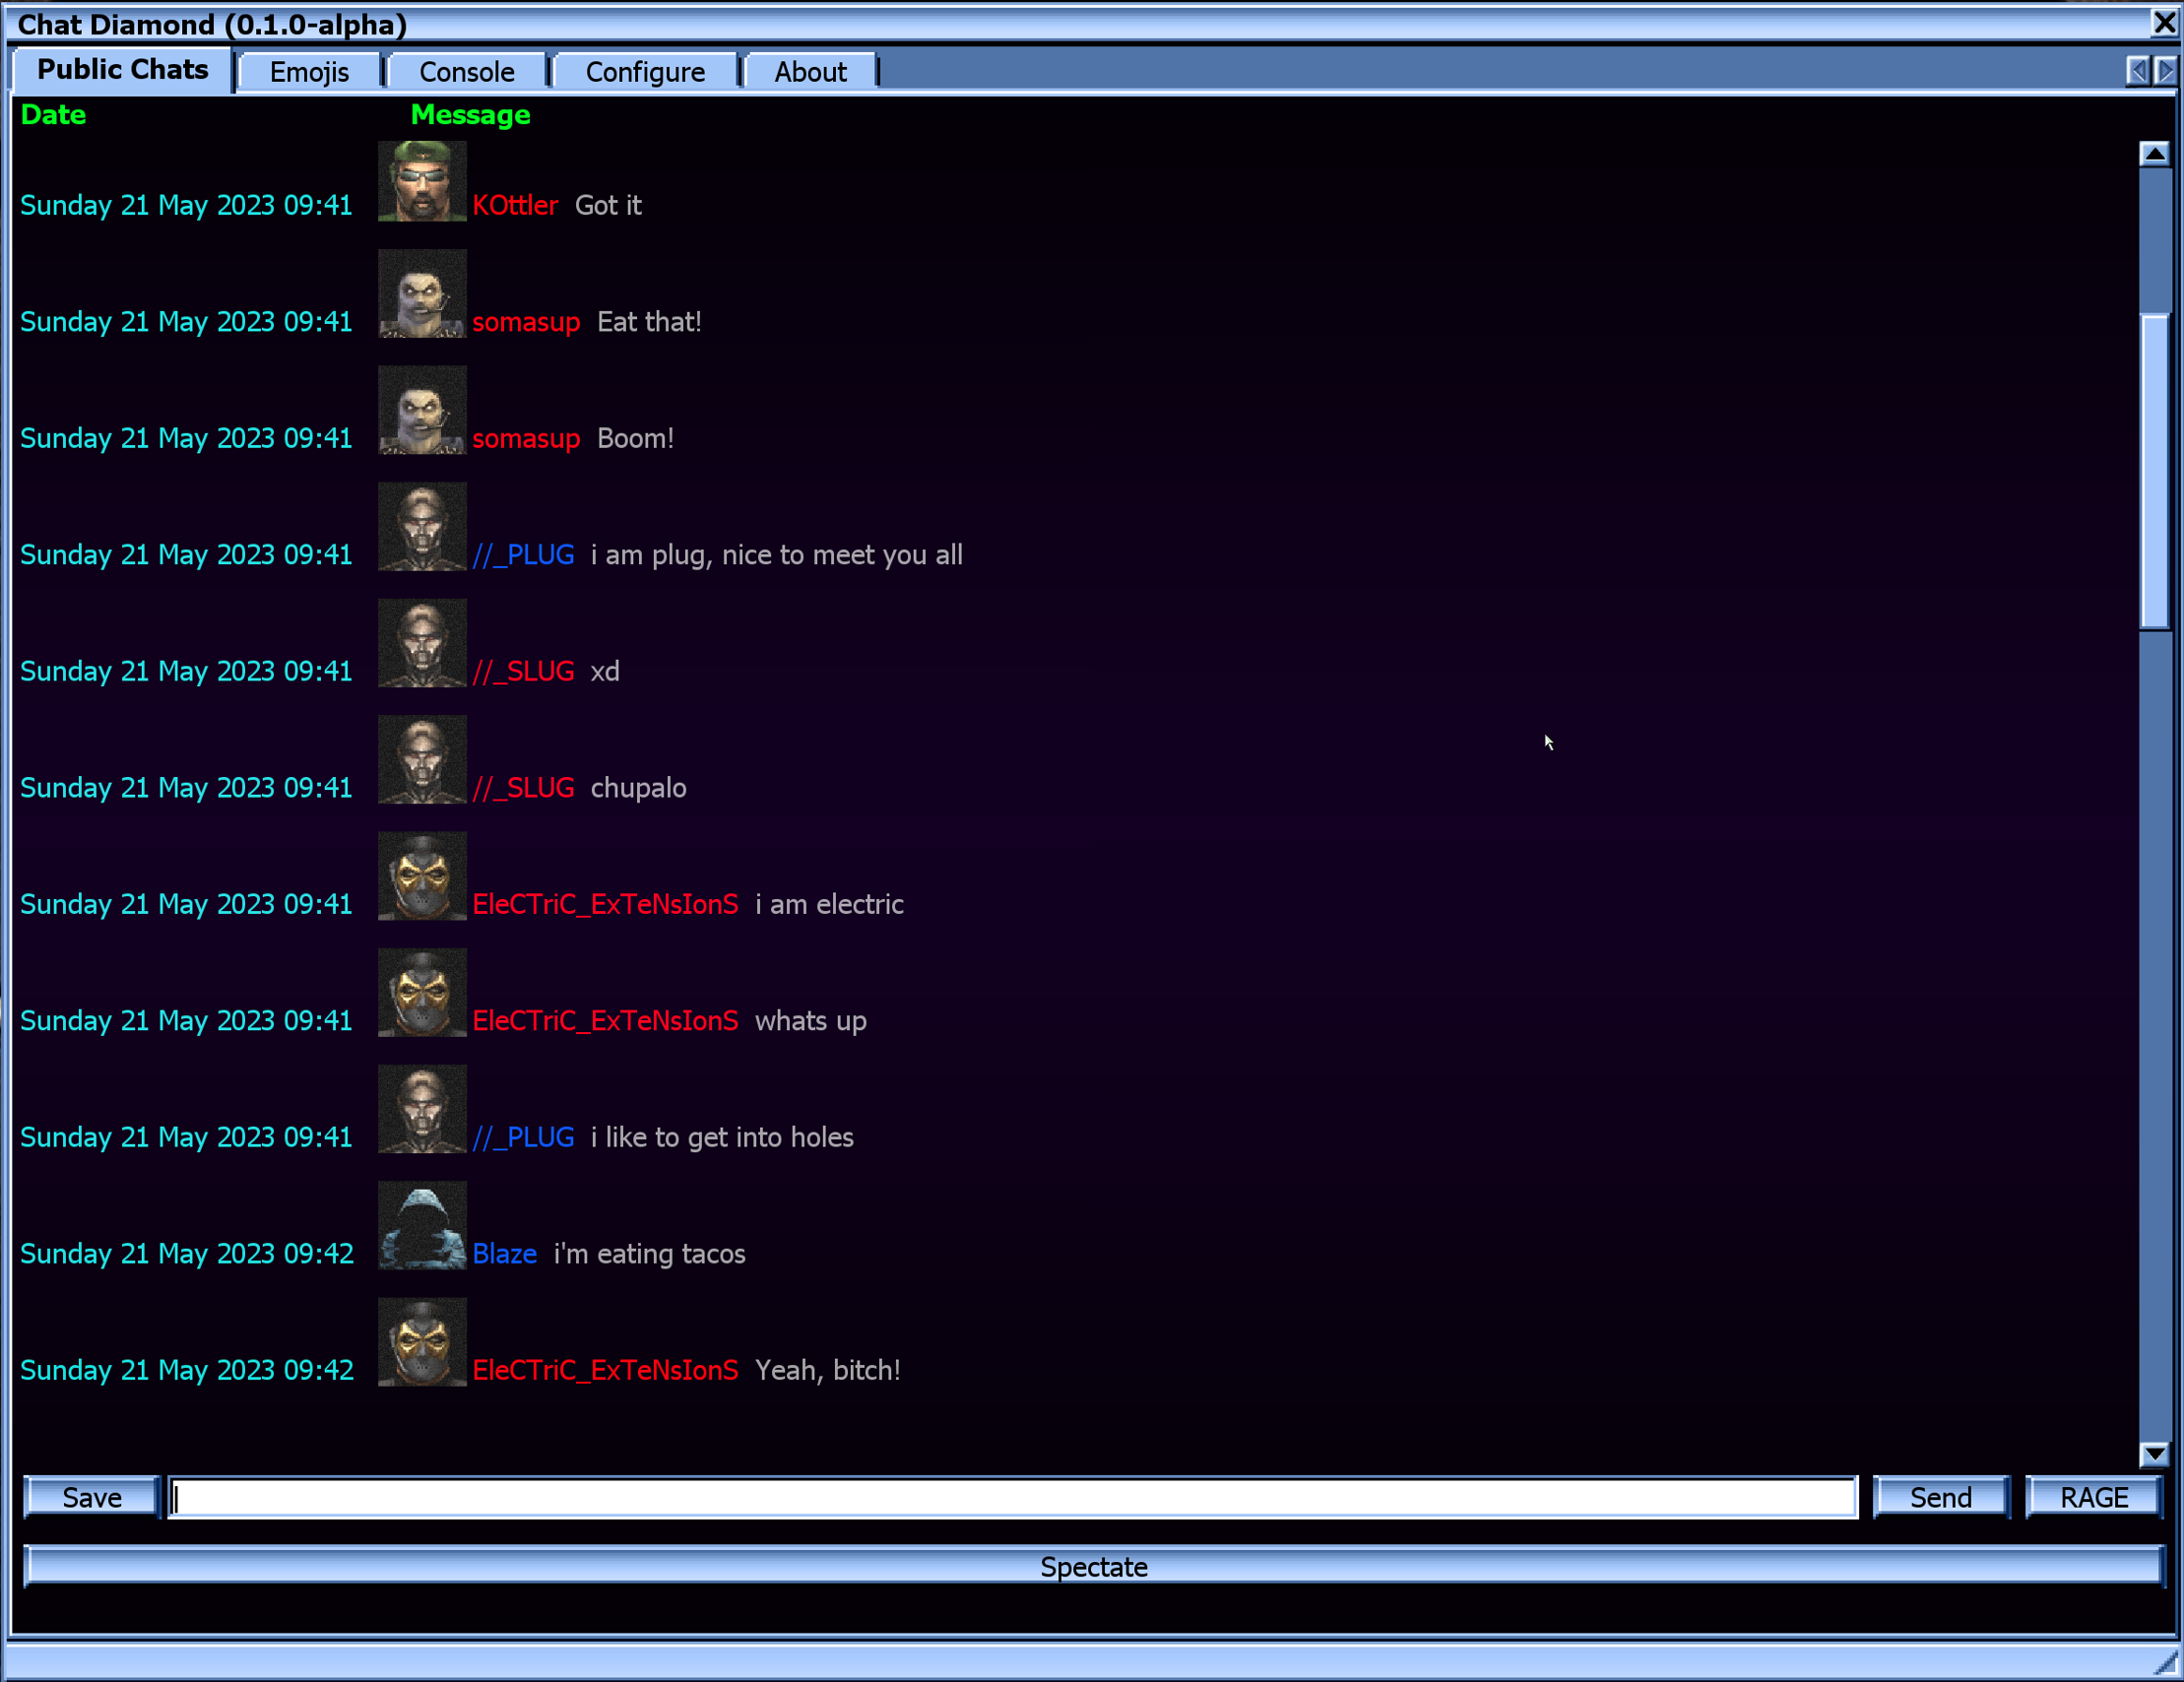
\includegraphics[width=0.4\textwidth]{img}
\caption{A screenshot of the ChatDiamond \ChatDiamondVersion~chat}
\end{figure}

\subsection{Chat Window}
Figure \ref{fig:chatdiamond} shows the current form of the chat window. The following features are supported
\begin{itemize}
\item Display of sender's avatar face.
\item Static emojis and animated emotes.
\item Display of Date and Time (long format for now).
\item Display of the Server name for reference purposes.
\end{itemize}

\subsection{Console Window}
\begin{figure}
\centering
\label{fig:chatdiamond_console}
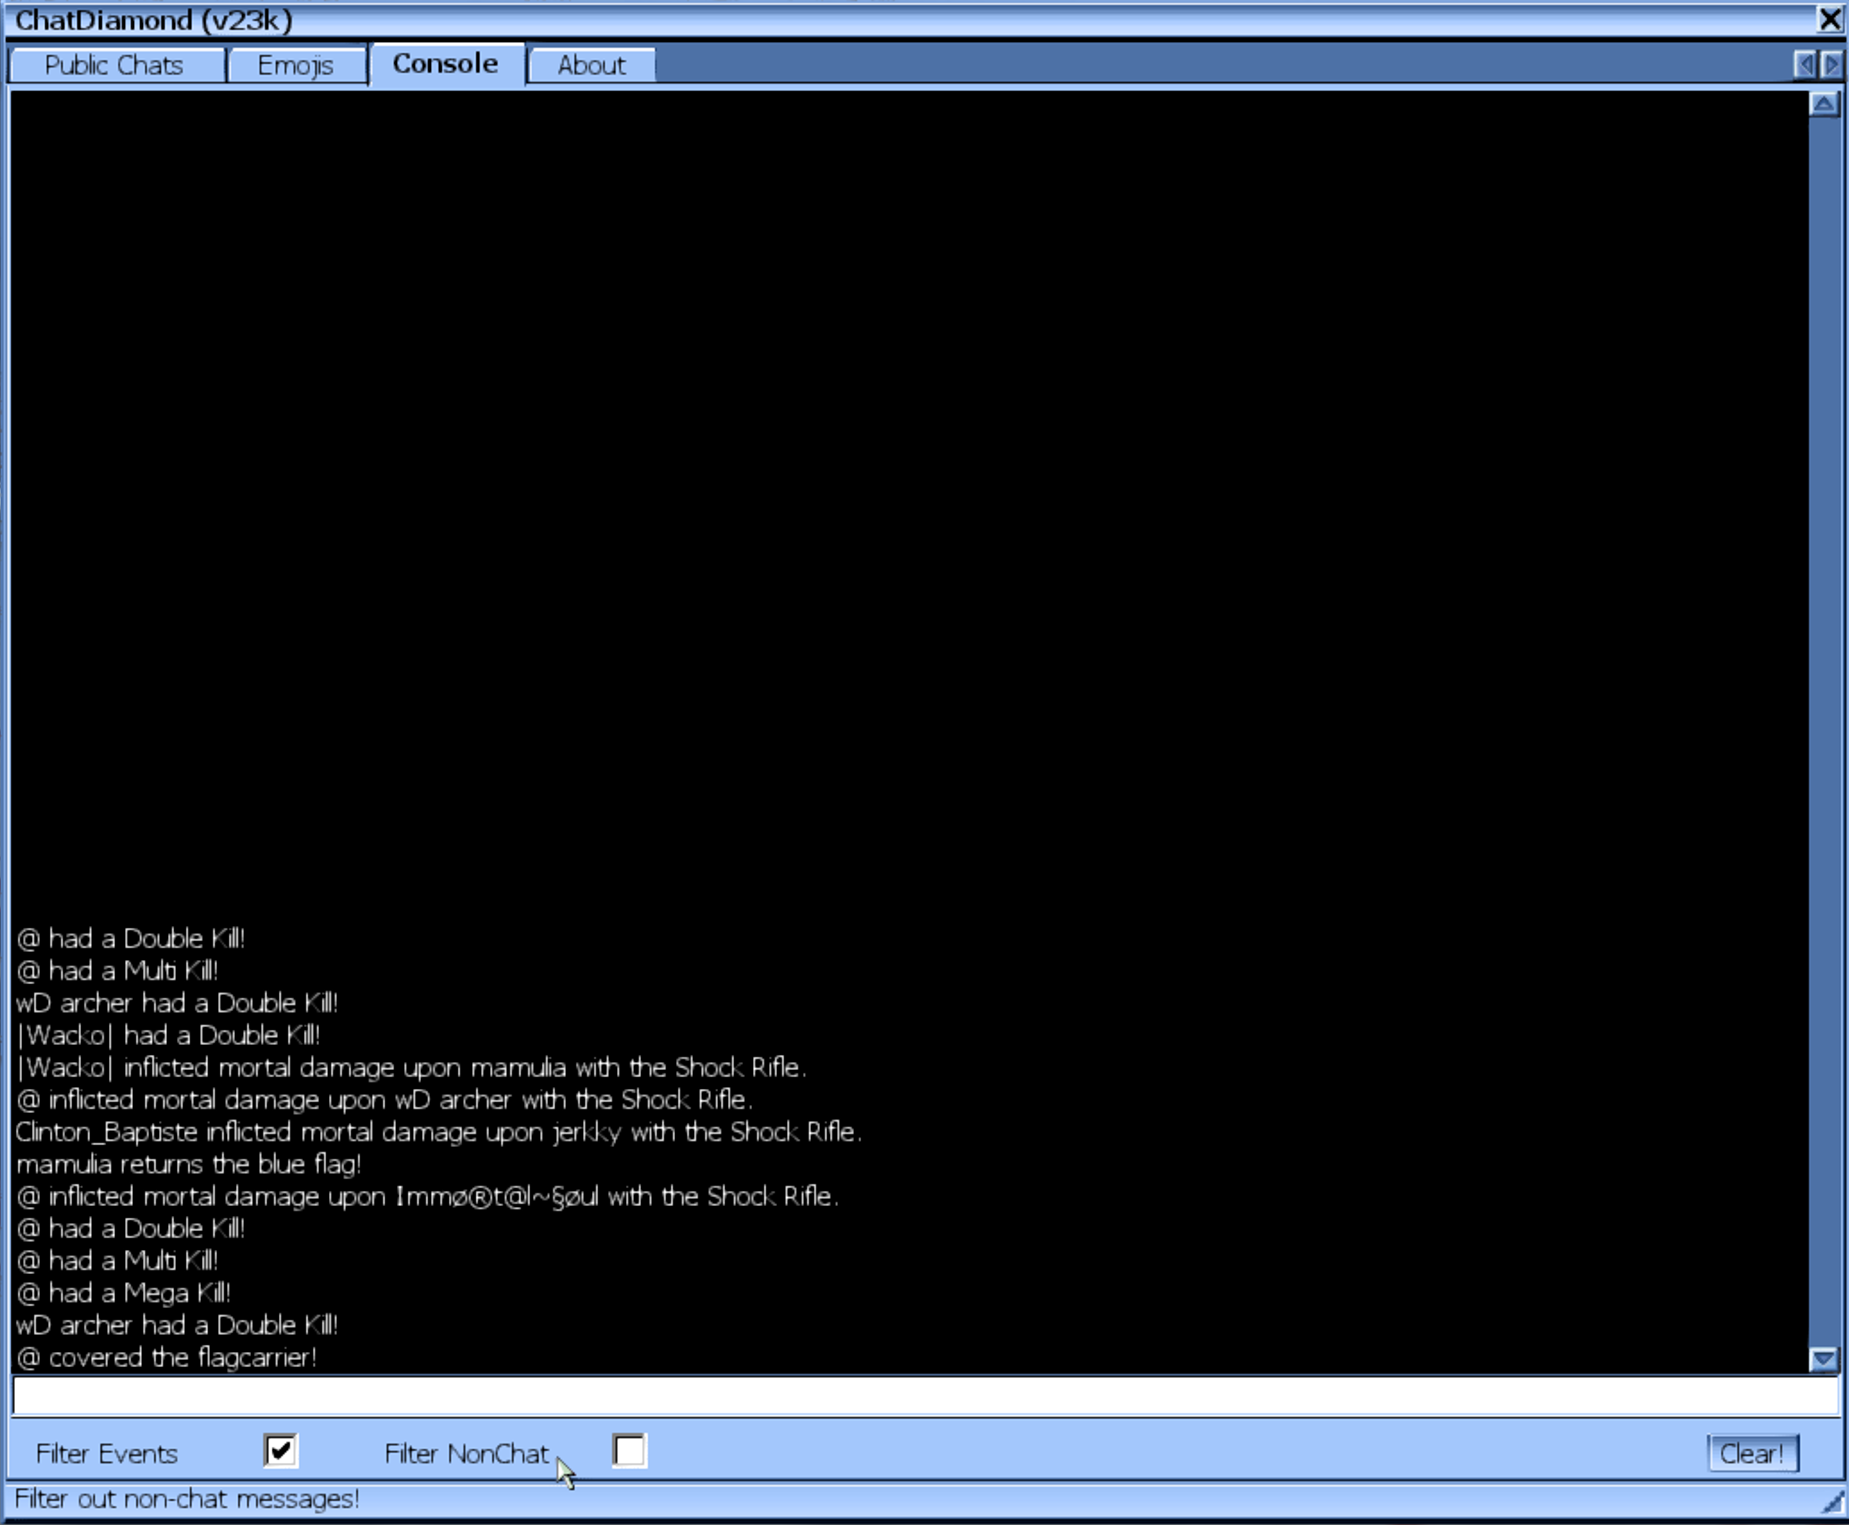
\includegraphics[width=0.4\textwidth]{img_console}
\caption{ChatDiamond \ChatDiamondVersion~console}
\end{figure}

The console now has the following features
\begin{itemize}
\item Non-chat filter to filter out server or mutator advertisements, in the console. Although SmartCTF cover and seal messages may also get filtered.
\item Event filter censors death messages corresponding to the weapon used.
\item A clear button to clean or reset the console.
\item A working status bar linked with console configuration modifiers.
\end{itemize}

\section{Installation}
ChatDiamond is developed and tested with UT 469c client.  Although the mod should work on previous versions, I take no pains for maintaining that code simply because I feel that we all should work towards pushing forward the community effort in driving the game (and UE 1) towards modern experience.  So by not supporting the code for earlier versions I am supporting the later versions.

With that being written, feel free to send pull requests to \href{https://github.com/ravimohan1991/ChatDiamond/}{ChatDiamond} repository, even for ealier game versions.

ChatDiamond is essentially a console (and not for the server).  So open for installation do the following
\begin{itemize}
\item Open {\color{Purple}UnrealTournament.ini} and find the section \\

\fbox{%
    \parbox{\textwidth}{%
       [Engine.Engine]\\
       GameRenderDevice=VulkanDrv.VulkanRenderDevice\\
       AudioDevice=ALAudio.ALAudioSubsystem\\
        \ldots  \\       
       {\color{Green}Console=UTMenu.UTConsole}\\
       \ldots        
    }%
}
\\

\item Modify to \\

\fbox{%
    \parbox{\textwidth}{%
        \ldots  \\       
       {\color{Green}Console=ChatDiamond.CDUTConsole}\\
       \ldots        
    }%
}
\\

\item And that is it!  You can now summon console by usual `$\sim$' key.

\subsection{Configuration}
I am not providing {\color{purple}ChatDiamond.ini}, which should be generated after first successful run of the mod.  

Once that is done make sure to configure the file.

\end{itemize}

\section{A note on UT Messaging}
ChatDiamond's functionality is based upon the tenet ``A complete clientside user interface with no dependencies with the server''.  This would imply conforming to the UT standards and any server not conforming to the standards, if so, is not worth visiting.

Based upon the above motivation we have a choice to make between replacing the client HUD or UT console, in order to gather the UT messages clientside.  My first instinct was to replace the HUD because that would give more precise classification of the messages, in the sense Epic wrote the code, like \href{http://uncodex.ut-files.com/UT/v436/Source_botpack/challengehud.html}{so} (line 1499)

\begin{lstlisting}[frame=single]
// Entry point for string messages.
simulated function Message( PlayerReplicationInfo PRI, coerce string Msg, name MsgType )
{
    local int i;
    local Class<LocalMessage> MessageClass;

    switch (MsgType)
    {
        case 'Say':
        case 'TeamSay':
            MessageClass = class'SayMessagePlus';
            break;
        case 'CriticalEvent':
            MessageClass = class'CriticalStringPlus';
            LocalizedMessage( MessageClass, 0, None, None, None, Msg );
            return;
        case 'DeathMessage':
            MessageClass = class'RedSayMessagePlus';
            break;
        case 'Pickup':
            PickupTime = Level.TimeSeconds;
        default:
            MessageClass = class'StringMessagePlus';
            break;
     }
   %* \ldots *)           
\end{lstlisting}

The basic premise of many cheats providing aim assist is to modify the HUD clientside and display the adversary's position behind the wall or a radar.  This is the reason why modern anticheats are not receptive of clients modifying HUD, and thus, work with the concept of ``whitelisting''.

If the notion of ``cheat-anticheat'' interplay exists in the UT standards, then that simply doesn't fit with the tenant we began with.  We don't want to be sending request to server administrators for specifically whitelisting ChatDiamond which will be reverted by cold silent treatment to say the most and some naggy jibber jabber about the unknown-ness of ChatDiamond, especially when the mod is not that popular.

So with this thiking in mind, the better option would be to replace the client console, which I haven't seen any anticheat scanning. This not only gets the client out of hook for sending whitelisting requests but also provides a powerful mechanism to mould the console, specificifically for generic needs (see the concept of \emph{filters}).

\subsection{A minor PhD on console messages}

We start with the \href{http://uncodex.ut-files.com/UT/v436/Source_engine/playerpawn.html}{code} 

\begin{lstlisting}[frame=single]
event ClientMessage( coerce string S, optional Name Type, optional bool bBeep )
{
     %* \ldots *)    
    if (Player.Console != None)
        Player.Console.Message( PlayerReplicationInfo, S, Type );
    if (bBeep && bMessageBeep)
        PlayBeepSound();
    if ( myHUD != None )
        myHUD.Message( PlayerReplicationInfo, S, Type );
}       
\end{lstlisting}
and
\begin{lstlisting}[frame=single]
event TeamMessage( PlayerReplicationInfo PRI, coerce string S, name Type, optional bool bBeep  )
{
    if (Player.Console != None)
        Player.Console.Message ( PRI, S, Type );
    if (bBeep && bMessageBeep)
        PlayBeepSound();
    if ( myHUD != None )
        myHUD.Message( PRI, S, Type );
}     
\end{lstlisting}

It is clear that both the console and HUD should receieve same messages with no discrimination (unless if coder specifically demands, as mentioned in \ref{foot:hudconsolediff}).  The console would display them, in what I would like to think, \emph{raw} form.  The diff, between console and HUD, is shown in the figure \ref{fig:chatdiamond_console_hud}

\begin{figure}
\centering
\label{fig:chatdiamond_console_hud}
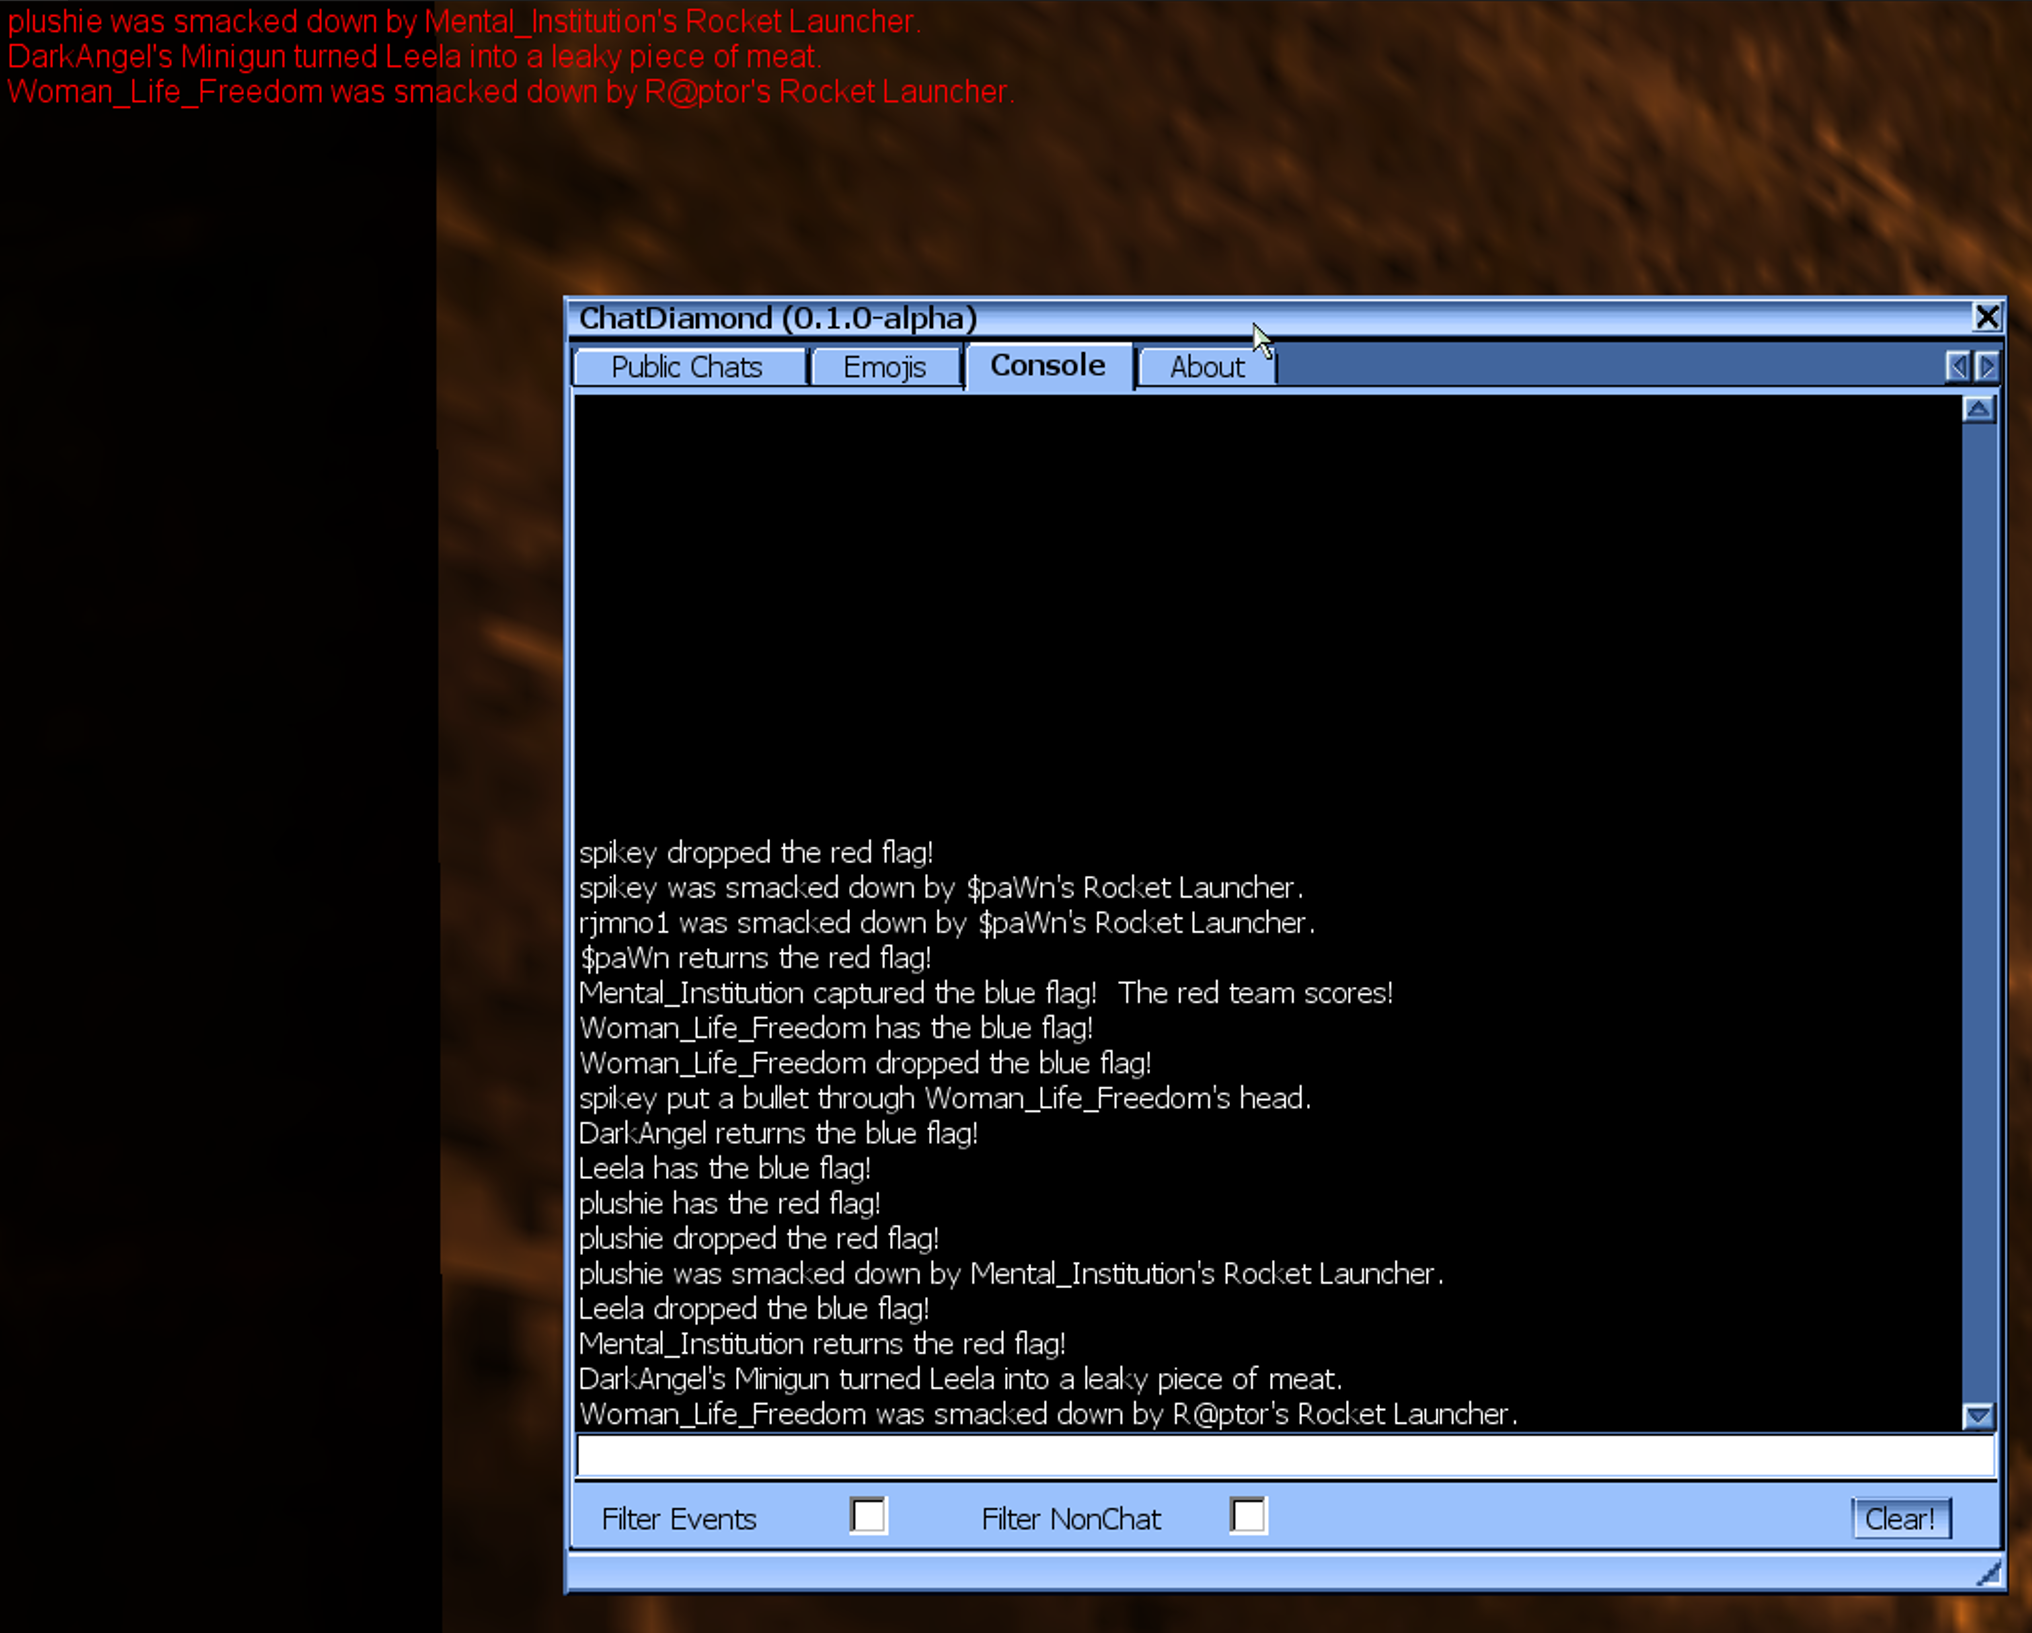
\includegraphics[width=0.4\textwidth]{consoleundhud}
\caption{UT99 HUD with ChatDiamond console}
\end{figure}

Please note that ChatDiamond's console is not much different from default UT99 visually.  The changes are how ChatDiamond interprets the raw messages thrown and utilize them in a constructive way. So this is where magic \href{https://github.com/ravimohan1991/ChatDiamond/blob/859323fbd80266b21c9dab163b067cacfa318463/Classes/CDUTConsole.uc#L52-L71}{code} comes in.  In order to understand that let me first demonstrate UT messaging by a table\footnote{\label{foot:hudconsolediff} The ``messages'' for instance: `plushie was smaked down by Mental\_Instituitions's Rocket Launcher', are actually strings which can be seen in the line 117 of the \href{http://uncodex.ut-files.com/UT/v436/Source_botpack/deathmessageplus.html}{code}.  This also shows how some deathmessages can be suppressed in the console thus differing from HUD.}.

\begin{tabcontainer}
 \begin{tabularx}{\textwidth}{| X | X | X | X |}
 \hline
 \makecell{Console\\ Owner\\ State} & \makecell{Death\\ Messages}\footnote{A string rather.  See \ref{foot:hudconsolediff}}  & \makecell{Server\\ Announcements\footnote{Server adds?}} & \makecell{Talk \\ TeamTalk} \\ [0.5ex] 
 \hline\hline
 
\makecell{Multiplayer \\Spectator} & \makecell{\color{red}{plushie was}\\ \color{red}{smaked down}\\ \color{red}{by MI's}\\ \color{red}{Rocket Launcher}} & \makecell{Type !cg to\\ visit combogib\\ grapple server}  & \makecell{A: Self Sent- \\RN\footnote{Receiever's (who is spectator) Name}:Hola\\  \\ B. By Player-\\ RN:SN\footnote{Sender's name, who is a player.}:Hola \\ \\ C. By spectator\footnote{A different spectator}\\ SN:Hola}\\

\hline
  \end{tabularx}
  \caption{Table of Messages.}
  \label{tab:messform}
\end{tabcontainer}

The mapping to relevant arguments is like so

\begin{tabcontainer}
 \begin{tabularx}{\textwidth}{| X | X | X | X |}
 \hline
 \makecell{Console\\ Owner\\ State} & \makecell{Death\\ Messages}\footnote{A string rather.  See \ref{foot:hudconsolediff}}  & \makecell{Server\\ Announcements\footnote{Server adds?}} & \makecell{Talk \\ TeamTalk} \\ [0.5ex] 
 \hline\hline
 
\makecell{Multiplayer \\Spectator} & \makecell{MessageType:  \\ DeathMessage?\\ \\ PRI:  Local?} & \makecell{MessageType:\\ Event \\  \\ PRI: Local}  & \makecell{A. \\ MessageType:\\ Event  \\ PRI: Local \\ \\  B.\\ MessageType: \\ Event \\ PRI: local\\ \\ C. \\  MessageType: \\ Event \\ PRI: Local}\\
    \hline

\makecell{Multiplayer\\ Player} & \makecell{Message Type: \\ Event \\ PRI: Local? } & \makecell{Message Type: \\ Event \\ PRI: None} & \makecell{A. \\ MessageType: \\ Say\\ PRI: Local\\ \\ B. \\ MessageType: \\ Say \\ PRI: SenderPRI \\ \\ C. \\ MessageType: \\ ? \\ PRI: ?}\\
    \hline
  \end{tabularx}
  \caption{Table of argument types.}
  \label{tab:messform}
\end{tabcontainer}

 

\end{document}